\chapter{Théorie}
Dans cette section sera présenté les prérequis et un état des lieux de l'apprentissage de la programmation aux enfants dans le monde. En premier lieu, il y aura les prérequis et SNAP BYOB. Ensuite un analyse des autres initiatives similaires à celle de ce travail. Suite à cela vendra la position du projet RSNAP par rapport à ce qui est déjà existant et expliqué dans les points précédent suivit d'une présentation des outils utilisés. La dernière partie portera sur ce qu'apport RSNAP par rapport aux autres projets existant.

\chapter{Connaissances nécessaires}
Ce chapitre commencera par présenter de manière succincte les prérequis pour pouvoir suivre ce document. Ensuite, une description plus technique présentera les outils utilisés.

\section{Prérequis}
Les connaissances nécessaires à la bonne compréhension de ce travail vont être développées dans cette partie.

\paragraph{Snap!}
Commençons par la partie portant sur Snap! BYOB. Cette application est implémentée en JavaScript. Donc, de bonnes connaissances dans ce langage de programmation seront un atout pour comprendre les apports et modifications de la version de départ. Des connaissances en XML et JSON seront également un plus pour toutes les fonctions d'importation et d'exportation.

\paragraph{Ruby on Rails}
La plateforme web, elle est implémentée en Ruby on Rails qui est le framework le plus utilisé pour la création de site web en Ruby. Ce framework est un atout car il permet de créer facilement des sites sur une architecture de type modèle-vue-contrôleur. Rails se base sur des conventions au lieu de se baser sur des configurations. Cela permet d'alléger considérablement le nombre de lignes nécessaires pour la création d'un site web. Ce framework étant basé sur Ruby, il permet l'usage des gems Ruby. Un gems est une bibliothèque logicielle qui permet d'avoir facilement des fonctionnalités supplémentaires. Plus de détails techniques seront donnés dans la suite de ce chapitre \ref{techno}. %TODO ajouter gem au glossaire

\paragraph{Pédagogie}
Pour l'apprentissage de la programmation aux jeunes, des notions de pédagogie sont également nécessaires. 
Les programmes d'apprentissages existants permettent de définir pour chaque année d'étude, les concepts considérés comme acquis par les élèves. La communication avec les jeunes demande un vocabulaire adapté. Tout ceci s'avère important pour les choix de design d'interface. Par exemple, suivant leur âge, les jeunes ne seront pas stimulés par les mêmes images ou couleurs. %TODO revoir ce chapitre

\subsection{Logiciel utilisé}
\subsubsection{Snap!}
\url{http://snap.berkeley.edu/SnapManual.pdf}
Cet partie va donner un aperçu de l'application réutilisée dans ce travail, à savoir Snap!. Comme dit précédemment, cette application est réalisée en JavaScript. La présentation de Snap! va se diviser en plusieurs partie. La première expliquera les différents types de blocs et comment ils sont implémentés. L'exécution d'un programme est l'étape suivante. Enfin, il sera présenté comment l'application affiche les différents éléments la constituant.

\paragraph{Blocs}
Il existe plusieurs type de blocs qui constitue un programme Snap!. Sur l'exemple de programme \ref{fig:software_used_script}, les différents types blocs disponible sont présentés.
\begin{figure}
  \begin{center}
    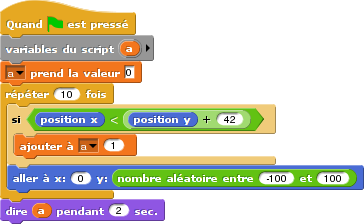
\includegraphics[width=0.5\textwidth]{content/4-theory/2-related_work/images/script}
    \caption{Exemple de programme Snap!}
    \label{fig:software_used_script}
  \end{center}
\end{figure}

\subparagraph{Commande}
Le type principal de bloc est \texttt{commande}. Ces blocs peuvent être compris comme étant des procédures. En effet, les blocs exécutes une ou plusieurs opérations sur le système en fonction des paramètres passés. Ces différents blocs doivent se baser soit sur une implémentation JavaScript pour les commandes élémentaires, soit être une composition de commandes pour fournir une commande plus complexe et/ou abstraite.

Dans l'exemple \ref{fig:software_used_script}, ce sont tout les blocs qui on la forme d'une pièce de puzzle. On peut voir que l'on a une succession de commandes qui crée un script. Les commandes ont plusieurs couleurs suivant la catégorie à laquelle elles appartiennent : mouvement, apparence, contrôles, variable, etc\ldots

\subparagraph{Reporter}
Les reporters sont des fonctions. En effet, ils retournent une valeur. Ils sont toujours utilisés en temps que paramètres d'un autre bloc. La plupart des reporter sont des accesseurs à des variables ou à des états du système (position souris, heure, etc\ldots). 

Les reporters sont les blocs de forme arrondie. L'exemple \ref{fig:software_used_script} montre différente utilisation de reporters : somme, valeur aléatoire, position \ldots Tout comme pour les commandes, les reporters peuvent être de différentes couleurs suivant leur catégorie.

\subparagraph{Prédicat}
Les prédicats sont des reporters qui retournent une valeur booléenne. Ils sont donc utilisés en conjonction avec des commandes demandant une condition.

Les prédicats sont les blocs de forme hexagonale.

\subparagraph{Chapeau}
Les chapeaux sont des commandes spéciales car ils sont le point d'entrée obligatoire d'un script. Ils permettent de démarrer l'exécution d'un script quand un événement se produit.

L'événement qui lancera le script \ref{fig:software_used_script} est donc le démarrage du programme. Celui-ci est symbolisé par un bouton avec drapeau vert.

\paragraph{Programme}
Snap! est plus qu'une interface graphique permettant de construire un programme. L'analyse du fonctionnement interne est l'objet de cette section.

Un programme est constitué de plusieurs processus. Chaque processus sera exécuté en parallèle grâce à un ordonnanceur.

% /*
%     A Process is what brings a stack of blocks to life. The process
%     keeps track of which block to run next, evaluates block arguments,
%     handles control structures, and so forth.
% 
%     The ThreadManager is the (passive) scheduler, telling each process
%     when to run by calling its runStep() method. The runStep() method
%     will execute some number of blocks, then voluntarily yield control
%     so that the ThreadManager can run another process.
% 
%     The Scratch etiquette is that a process should yield control at the
%     end of every loop iteration, and while it is running a timed command
%     (e.g. "wait 5 secs") or a synchronous command (e.g. "broadcast xxx
%     and wait"). Since Snap also has lambda and custom blocks Snap adds
%     yields at the beginning of each non-atomic custom command block
%     execution, and - to let users escape infinite loops and recursion -
%     whenever the process runs into a timeout.
% 
%     a Process runs for a receiver, i.e. a sprite or the stage or any
%     blocks-scriptable object that we'll introduce.
% 
%     structure:
% 
%     topBlock            the stack's first block, of which all others
%                         are children
%     receiver            object (sprite) to which the process applies,
%                         cached from the top block
%     context                the Context describing the current state
%                         of this process
%     homeContext            stores information relevant to the whole process,
%                         i.e. its receiver, result etc.
%     isPaused            boolean indicating whether to pause
%     readyToYield        boolean indicating whether to yield control to
%                         another process
%     readyToTerminate    boolean indicating whether the stop method has
%                         been called
%     isDead              boolean indicating a terminated clone process
%     timeout                msecs after which to force yield
%     lastYield            msecs when the process last yielded
%     errorFlag            boolean indicating whether an error was encountered
%     prompter            active instance of StagePrompterMorph
%     httpRequest         active instance of an HttpRequest or null
%     pauseOffset         msecs between the start of an interpolated operation
%                         and when the process was paused
% */

Un processus \texttt{Process} représente l'exécution d'un script, une pile de blocs. Il assure le suivit de l'exécution du script : prochain bloc à exécuter, objet sur lequel il s'applique (lutin, stage), contexte décrivant l'état courant \ldots

L'ordonnanceur \texttt{ThreadManager} appelle successivement la fonction \texttt{runStep()} (\ref{lst-runstep}) sur chaque processus. Cette fonction exécute un certain nombre de blocs via \texttt{this.evaluateContext()} de manière atomique. Elle rend la main volontairement à l'ordonnanceur quand elle a fini. Comme il est possible d'écrire soi-même des blocs, \texttt{runStep()} rend aussi la main si trop de temps s'est écoulé depuis le début de l'exécution de cette étape. La convention est que les processus rendent la main à la fin de chaque itération de boucle ou quand une opération relative au temps (attendre xxx secondes) ou synchrone (envoyer à tous xxx et attendre la réponse) est exécutée.

\begin{lstlisting}[caption={Fonction \texttt{runStep()} de \texttt{Process}},label=lst-runstep,language=JavaScript]
Process.prototype.runStep = function () {
/*
    a step is an an uninterruptable 'atom', it can consist
    of several contexts, even of several blocks
*/
    // allow pausing in between atomic steps:
    if (this.isPaused) {
        return this.pauseStep();
    }
    this.readyToYield = false;
    while (!this.readyToYield
            && this.context
            && (this.isAtomic ? (Date.now() - this.lastYield < this.timeout) : true) ) {
        // also allow pausing inside atomic steps - for PAUSE block primitive:
        if (this.isPaused) {
            return this.pauseStep();
        }
        this.evaluateContext();
    }
    this.lastYield = Date.now();

    // make sure to redraw atomic things
    if (this.isAtomic &&
            this.homeContext.receiver &&
            this.homeContext.receiver.endWarp) {
        this.homeContext.receiver.endWarp();
        this.homeContext.receiver.startWarp();
    }

    if (this.readyToTerminate) {
        while (this.context) {
            this.popContext();
        }
        // pen optimization
        if (this.homeContext.receiver &&
                this.homeContext.receiver.endWarp) {
            this.homeContext.receiver.endWarp();
        }
    }
};
\end{lstlisting}



% /*
%     A Context describes the state of a Process.
% 
%     Each Process has a pointer to a Context containing its
%     state. Whenever the Process yields control, its Context
%     tells it exactly where it left off.
% 
%     structure:
% 
%     parentContext    the Context to return to when this one has
%                     been evaluated.
%     outerContext    the Context holding my lexical scope
%     expression        SyntaxElementMorph, an array of blocks to evaluate,
%                     null or a String denoting a selector, e.g. 'doYield'
%     receiver        the object to which the expression applies, if any
%     variables        the current VariableFrame, if any
%     upvars          the current UpvarReference, if any (default: null)
%     inputs            an array of input values computed so far
%                     (if expression is a    BlockMorph)
%     pc                the index of the next block to evaluate
%                     (if expression is an array)
%     startTime        time when the context was first evaluated
%     startValue        initial value for interpolated operations
%     activeAudio     audio buffer for interpolated operations, don't persist
%     activeNote      audio oscillator for interpolated ops, don't persist
%     isLambda        marker for return ops
%     isImplicitLambda    marker for return ops
%     isCustomBlock   marker for return ops
%     emptySlots        caches the number of empty slots for reification
% */

\paragraph{GUI}
Un autre élément intéressant à analyser chez Snap! est sa façon d'afficher quelque chose dans la balise html \texttt{canvas}. Toutes les fonctionnalités de base nécessaire à afficher tout éléments graphiques (text rendering, blinking cursors, entry fields, menus, buttons, sliders, windows and dialog boxes \ldots) de Snap! découle de l'implémentation que l'on retrouve dans \texttt{morphic.js}.

\texttt{morphic.js} fournit les abstractions nécessaires à redessiner des parties de l'interface et pour interagir avec l'utilisateur. Le canvas utilisé possède un \texttt{world}. Ce \texttt{world} est la racine de l'arbre composé de \texttt{morph} et leur sous-\texttt{morph}. Chaque \texttt{morph} peut être déplacé, redimensionné via le code ou les manipulations de l'utilisateur.

L'idée principale de \texttt{morphic.js} est de continuellement parcourir tout les éléments du \texttt{world} pour redessiner ceux qui ont été modifié. Le \texttt{world} permet à l'ordonnanceur d'exécuter une étape entre chaque itération. L'exemple \ref{lst-doonecycle} que le monde est rafraîchit toutes les 50 millisecondes.

\begin{lstlisting}[caption={Exemple d'utilisation de \texttt{morphic.js}},label=lst-doonecycle,language=HTML5,alsolanguage=JavaScript]
<!DOCTYPE html>
<html>
    <head>
        <title>Morphic!</title>
        <script type="text/javascript" src="morphic.js"></script>
        <script type="text/javascript">
            var world;

            window.onload = function () {
                world = new WorldMorph(
                    document.getElementById('world'));
                setInterval(loop, 50);
            };

            function loop() {
                world.doOneCycle();
            }
        </script>
    </head>
    <body>
        <canvas id="world" tabindex="1" width="800" height="600" />
    </body>
</html>
\end{lstlisting}

La fonction \texttt{drawNew()} sert dessiner un \texttt{morph}. L'exemple \ref{lst-drawnew} montre que cette fonction dessine son objet sur une image stockée dans l'objet. Cette image provient d'un canvas virtuel généré grâce à l'image du \texttt{morph} parent.

\begin{lstlisting}[caption={Modèle pour la fonction \texttt{drawNew()}},label=lst-drawnew,language=JavaScript]
MyMorph.prototype.drawNew = function() {
    var context;
    this.image = newCanvas(this.extent());
    context = this.image.getContext('2d');
    // use context to paint stuff here
};
\end{lstlisting}

\subsubsection{Rails}
Rails est une plat-forme de développement d'application web basé sur le langage de programmation Ruby. Cette partie présente Rails au travers de sa philosophie, de son architecture et de ses environnements de tests.

\paragraph{Philosophie}
Rails fait l'assomption qu'il existe une meilleur façon d'aborder la création d'application web. Si le programmeur respect ce "Rails way", il améliorera sa productivité et écrira moins de code. D'après Rails, si il persiste à utiliser ses anciennes habitudes, le développeur s'amusera beaucoup moins en développant son application.

Pour atteindre cet objectif, Rails utilise deux principes majeurs :
\begin{description}
  \item[Convention plutôt que configuration] (CoC) Pour permettre au programmeur d'écrire moins de code, Rails permet de n'écrire que ce qui ne correspond pas aux conventions. Rails utilise la méta-programmation pour fournir les conventions à tous les objets;
  \item[Ne vous répétez  pas] (DRY) L'architecture que propose Rails permet de mettre l'information à un endroit unique et bien déterminé. Ceci permet d'avoir un code plus court, plus maintenable, plus extensible et avec moins de bugs.
\end{description}

\paragraph{architecture}
Rails se base sur une architecture Modèle-Vue-Contrôleur.
\subparagraph{Modèle} 
Un modèle est typiquement une classe qui représente une table de la base de données. Une classe du modèle fournit aussi toutes les méthode nécessaire à représenter et modifier l'objet dans le domaine d'application.

La correspondance entre un objet Ruby et la base de données est réalisée grâce à Active Record. Ce module de Rails permet de faire des appels sur des objets Ruby alors que dans d'autres framework, il faudrait utiliser des requêtes SQL.
  
\subparagraph{Contrôleur} 
Le contrôleur permet d'accéder à une ressource. Une ressource est un modèle ou tout autre objet plus indirect (enregistrement/login, page d'accueil\ldots).  

Il détermine quelle vue doit s'afficher et avec quel paramètre. Le contrôleur a donc la tache de vérifier la sécurité et l'intégrité des données fournies par l'utilisateur. Ensuite, il peut interroger différents modèles et fournir les réponses à la vue adéquate. 

Rails encourage d'avoir des ressources REST. C'est a dire, d'avoir des ressources avec une représentations unique et des actions identiques (create, new, edit, update, destroy, show, index). Les actions disponibles sur un contrôleur sont déterminées via le fichier de configuration des routes.

\subparagraph{Vue} 
Les vues sont ce que les utilisateurs reçoivent et voient. Ce sont typiquement des pages html mais aussi des pdf, objets json, fichiers, etc\ldots 

La philosophie de Rails est d'utiliser des gems pour simplifier l'écriture. Pour les vues, nous avons notamment:
\begin{description}
  \item[Haml] un langage fournissant une syntaxe raccourcie du html. Il se base sur l'indentation plutôt que sur une syntaxe XML. Haml permet donc de respecter le principe DRY et d'amélioré la lisibilité par code plus court et bien indenté;
  \item[JQuery] Cette bibliothèque javaScript bien connue permet de modifier le document courant facilement, de géré des événements, de crée des annimation, etc\ldots
  \item[CoffeeScript] Est un langage qui se compile en JavaScript. Il permet d'avoir une syntaxe plus claire et plus courte, il permet d'ajouter des sucre syntaxique par rapport à JavaScript;
  \item[Bootstrap] un framework CSS qui permet de découpler le fond de la forme de l'affichage d'une page html. Ce framework donne un design responsive pour tout type d'écran au page qui l'utilise. Il fournit aussi de nombreux composants utiles (boutons, alertes, barre de progression, message d'aide \ldots).
\end{description}

\paragraph{gem}
Ruby fourni de base une manière de partager des extenstions pour des programmes ruby via les gems. Rails est un gem et dépend de nombreux autres notament Active Record présenté plus haut.

La communauté de Rails à écrit de nombreux gems permettant de rajouter facilement des fonctionnalités à une application. Des gems intéressantes seraint les suivantes :
\begin{description}
  \item[Paperclip] permet de facilement récupérer et stoquer des fichiers. Paperclip permet donc d'intégrer la gestion de fichier tiers de manière propre dans une classe du modèle. Il fourni notament divers drivers pour stoquer ceux-ci aussi bien en local que sur le cloud d'amazon ou de dropbox.
  \item[devise] permet de gérer toute la problèmatique de l'autentification des utilisateurs.
  \item[rolify] permet de donner des rôles aux utilisateurs de manière générale (ex. administrateur) ou sur une ressource (ex. modérateur d'un forum).
  \item[autority] Permet de gérer les droits des utilisateurs sur les différentes ressources contrôleur.
\end{description}

\paragraph{test}
Il existe tout un écosystème autour de Rails pour fournir du code de qualité. %TODO faire une suite à l'intro\\

Un outil de test fort apprécié des programmeur Ruby et plus particulièrement Rails est Cucumber. Cucumber permet de réaliser des tests dans un "behavior-driven development" (BDD) style. Ce style de test permet d'une part au client ou chef de projet d'écrire des scénarii décrivant l'utilisation de fonctionnalité du domaine en langague naturel (Gherkin) et d'autre part au programmeur d'implémenter ceux-ci. Ce type de test permet de mettre l'accent sur ce que veux le client.

Dans le cas de Rails, il est intéressant d'utiliser conjointemant à Cucumber Capybara. Capybara permet de controler un navigateur et donc de réaliser des tests à la place d'un utilisateur. Ces tests permettrons donc bien d'assurer que ce que désire l'utilisateur fonctionne correctement.\\

Dans le cadre d'un développement actif, il est intéressant d'avoir un serveur qui réalise des tests d'intégration continue. Ce style de testing permet d'effectuer tout les tests sur le code à chaque nouveau commit. Cela permet de connaitre directement si une modification du code source à induit un régression des fonctionnalités.\\

Un autre outils permet de mieux comprendre et respecter le "Rails way" présenté plus tôt. rails\_best\_practices fournis des métriques utiles pour détecter des écarts à philosophie Rails. Cet outil s'utilise en association avec le conseil fournit par \url{http://rails-bestpractices.com} aidant à refactorer les morceaux de code qui ne respecterait pas les conventions.


\section{Travail associé}
Nous allons ici présenté un aperçu des initiatives similaire à Rsnap.
\subsection{Code.org}
Code.org\footnote{\url{http://code.org/about}} est une organisation sans but lucratif des USA qui à pour objectifs :
\begin{itemize}
  \item Apporter l'informatique dans toutes les classes de secondaire aux USA;
  \item Démontrer le succès de l'utilisation de cours en ligne dans l'enseignement public;
  \item Ajouter l'informatique dans les bases des programmes de sciences/math des 50 états;
  \item Employé la connaissance technique collective pour améliorer l'apprentissage de l'informatique dans le monde;
  \item Augmenter la représentation féminine et des personnes de couleurs dans informatique.
\end{itemize}

Pour ce faire, il fournisse une plat-forme\footnote{\url{http://code.org/educate/20hr}} web qui permet aux professeurs de suivre leur élèves grâce à un système de classe.

Toutes les ressources sont gratuites et librement utilisable\footnote{\url{http://code.org/faq}}. Leur programme d'apprentissage se base sur Blockly (voir \ref{blockly}).
Les ressources sont conçues pour que les professeurs comme les étudiants puissent commencer le cours sans connaître l'informatique (un assistance est proposé au professeur gratuitement si nécessaire).

Le site propose aux professeurs de se faire récompenser si ils arrivent à finir les 27 missions proposée à  minimum 15 étudiants. Dans ce cas ils gagnent $750\$$, si ils ont au moins 7 filles dans le groupe ils peuvent prétendre a $250\$$ supplémentaire.

\subsubsection{déroulement des lecons}
Il propose des session de une heure de travail/jeu/apprentissage. Chaque unité d'une heure est découper en petite mission (ex:5-20) les missions sont très courte et apporte un concept de programmation. Avant l'introduction de chaque concept une petite vidéo est faire pour expliquer le concept introduit et des exemples de ce que la programmation permet de réaliser avec ce dernier.

Ils proposent de faire travailler les étudiants par pair\footnote{pair programming \url{http://en.wikipedia.org/wiki/Pair\_programming}}. Ceci permet d'avoir moins de questions pour le professeur et de mieux s'approprier la matière. Le travail par pair permet également de casser l'image du "geek" en montrant que la programmation est une sciences sociale et collaborative. Sans oublier qu'avec deux enfants par station, moins d'ordinateurs seront nécessaire.

Le site explique également que pour faire participer tout les élèves, on avoir confiance en leur compétence : permettre aux premiers groupes d'aider les derniers.

Pour résoudre un problème, ils recommandent de proposer au étudiants de d'abord demander à 3 de leur camarades avant de poser la question au professeur. Le prof ne devant pas être compétent, il doit juste pouvoir réfléchir avec les élèves de quel est le problème, cela permet aussi d'évité les questions de distraction ou de manque de compréhension.

Pour chaque petite mission il y a un test automatisé qui dit si la mission est réussie ou non. Si la mission est réussie, le programme passe à la mission suivante. Il y a également un compteur de blocs dans les première mission. Ce compteur permet de voir combien de bloc sont nécessaire pour réaliser la mission de manière optimale.

\subsection{Blockly}
\label{blockly}


Blocky\footnote{\url{https://code.google.com/p/blockly/}} est un éditeur de programmation graphique basé sur des technologie du web. 

Blocky est influencé\footnote{\url{https://code.google.com/p/blockly/wiki/Alternatives}} par "App Inventor" qui est influencé par "Scratch". Ce dernier est lui influencé par "StarLogo".

Il a comme particularité:
\begin{enumerate}
\item De s'exécuter dans un navigateur;
\item D'exporter du code source en JavaScript, dart, etc..;
\item D'être open source;
\item D'être haut-niveau.
\end{enumerate}

Il n'est pas directement une plat-forme d'éducation dans le sens ou suivant les blocs implémenté, il sera utilisé pour l'éducation, le business, des jeux, etc..


Lors de la conception du language de blocky il devait avoir certaines propriétés. Les trois première sont pour augmenter la compréhension des néophyte, les autres portait sur des facilité souhaiter du langage. Les propriétés décidées lors de la conception du langage sont:\footnote{\url{https://code.google.com/p/blockly/wiki/Language}}:

\begin{itemize}
  \item Des index de liste commençant à 1;
  \item Des nom de variables non sensible à la casse;
  \item Pas de scoope de variable, toutes les variables sont globale;
  \item La possibilité de pouvoir faire un export en JavaScript;
  \item Un code natif généré proche de celui des blocs.
\end{itemize}

\section{CoderDojo}
CoderDojo\footnote{\url{http://coderdojo.com/about}} est un réseau open source de clubs de programmation dans le sens le plus large du terme. Tous les dojos sont donc autonome.  Dans ceux-ci, des enfant de 5 à 17 ans apprennent la programmation (site web, application, jeux...). la seul règle est  “Above All: Be Cool“ qui peut être mise en pratique simplement en créant des espace d'échanges de savoir amicale et sociable.

CoderDojo à été crée par James Whelton un irlandais de 18 ans et Bill Liao un entrepreneur australien à Cork. James a eu des demandes de jeunes enfants pour avoir des cours de programmation après qu'il eut hacké l'ipod nano. Pas mal de gens de Dublin vinrent à ses cours et donc un nouveau Dojo à été crée à Dublin et puis cela s'est étendu à tout le globe.

\section{Code Club}

Code Club\footnote{\url{https://www.codeclub.org.uk/about}} est un réseau de club national mené par des bénévole en dehors des heures de cours. Ces activités s'adressent à des enfants entre 9 et 11 ans.

Ils créent donc le matériel pour permettre à des bénévole de donner des cours parascolaire d'environ une heure semaine. Il propose dans l'ordre d'utiliser scratch, html/css et python. ils aimeraient que les 21 000 écoles primaires anglaises ai leur club.

Leur philosophie est de d'abord l'amusement, la créativité et l'exploration avant l'apprentissage des concept de programmation.

\section{L'état de la programmation dans le monde}
Nous allons ici faire un tour d'horizon de différent pays d'européen ou non qui enseignent la programmation aux jeunes. 
\subsection{England}

L'apprentissage de l'informatique en Angleterre\footnote{\url{https://www.gov.uk/government/collections/statutory-guidance-schools\#national-curriculum-from-september-2014}} n'est pas nouveau. Pendant longtemps cet apprentissage était centré sur les technologies de l'information et de la communication (TIC). En 2010 un étude a été commandée à la Royal Society pour évaluer cet apprentissage. Un an plus tard leur rapport a révélé que l'enseignement tel que dispensé jusque là, n'était ni efficace ni en adéquation avec l'évolution de l'informatique dans notre société. La Royal Society suggère de changer les matières abordées en informatique. En effet précédemment ce sont les TIC qui étaient prescrites. L'apprentissage de la programmation serai plus bénéfique et adapter pour les enfants. Sur base de ce rapport les programmes de cours ont été adaptés.


\subsection{France}
En France\footnote{\url{http://fr.wikipedia.org/wiki/Informatique\_et\_sciences\_du\_num\%C3\%A9rique}
\url{http://fr.wikipedia.org/wiki/Baccalaur\%C3\%A9at\_scientifique}} depuis deux an l'informatique fait partie intégrante du programme du baccalauréat de type S. Une des matière dispensée est "Informatique et sciences du numérique". Cette matière se subdivise en quatre sous parties qui sont : représentation de l'information, algorithmique, langage et programmation, architectures matérielles. Cette approche est donc également basé sur l'apprentissage de la programmation plutôt que sur les TIC.

\subsection{Nouvelle Zélande}
Ce pays à adopté récemment les sciences informatique dans sont programme d'étude. Les cours sont dispenser à partir de 15 ans. Les cours dispensé concerne l'apprentissage de la programmation et des concepts informatique en général. Nous avons un choix un peu différent dans ce pays sur l'âge du début de l'apprentissage. Beaucoup de pays commence plus jeune et introduise des concepts basiques. La Nouvelle Zélande s'inscrit dans une logique plus similaire à la France mais ne restreint pas l'informatique aux options scientifiques.

\subsection{Corée du Sud}
Enseigne l'informatique depuis longtemps et à tous les niveaux de l'enseignement. La culture numérique dans ces pays y est fort différent que par chez nous. Par exemple une carrière dans le gaming y est tout à fait normal. L'informatique est vraiment omni-présent dans ces cultures, il est donc normal que son apprentissage commence en primaire.

\subsection{Grèce}
L'apprentissage des sciences informatiques prend une place important dans les programme grec. Des 6 ans les enfants sont confronté à l'informatique à l'école. A cette age c'est plus de la maîtrise de l'outil qu'il apprennent. Dès 10 ans, leurs cours d'informatique prend une tournure plus algorithmique et donc plus proche de la computer sciences.


\subsection{Logiciel utilisé}
\subsubsection{Snap!}
\url{http://snap.berkeley.edu/SnapManual.pdf}
Cet partie va donner un aperçu de l'application réutilisée dans ce travail, à savoir Snap!. Comme dit précédemment, cette application est réalisée en JavaScript. La présentation de Snap! va se diviser en plusieurs partie. La première expliquera les différents types de blocs et comment ils sont implémentés. L'exécution d'un programme est l'étape suivante. Enfin, il sera présenté comment l'application affiche les différents éléments la constituant.

\paragraph{Blocs}
Il existe plusieurs type de blocs qui constitue un programme Snap!. Sur l'exemple de programme \ref{fig:software_used_script}, les différents types blocs disponible sont présentés.
\begin{figure}
  \begin{center}
    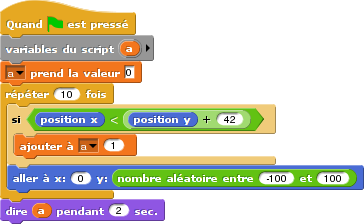
\includegraphics[width=0.5\textwidth]{content/4-theory/2-related_work/images/script}
    \caption{Exemple de programme Snap!}
    \label{fig:software_used_script}
  \end{center}
\end{figure}

\subparagraph{Commande}
Le type principal de bloc est \texttt{commande}. Ces blocs peuvent être compris comme étant des procédures. En effet, les blocs exécutes une ou plusieurs opérations sur le système en fonction des paramètres passés. Ces différents blocs doivent se baser soit sur une implémentation JavaScript pour les commandes élémentaires, soit être une composition de commandes pour fournir une commande plus complexe et/ou abstraite.

Dans l'exemple \ref{fig:software_used_script}, ce sont tout les blocs qui on la forme d'une pièce de puzzle. On peut voir que l'on a une succession de commandes qui crée un script. Les commandes ont plusieurs couleurs suivant la catégorie à laquelle elles appartiennent : mouvement, apparence, contrôles, variable, etc\ldots

\subparagraph{Reporter}
Les reporters sont des fonctions. En effet, ils retournent une valeur. Ils sont toujours utilisés en temps que paramètres d'un autre bloc. La plupart des reporter sont des accesseurs à des variables ou à des états du système (position souris, heure, etc\ldots). 

Les reporters sont les blocs de forme arrondie. L'exemple \ref{fig:software_used_script} montre différente utilisation de reporters : somme, valeur aléatoire, position \ldots Tout comme pour les commandes, les reporters peuvent être de différentes couleurs suivant leur catégorie.

\subparagraph{Prédicat}
Les prédicats sont des reporters qui retournent une valeur booléenne. Ils sont donc utilisés en conjonction avec des commandes demandant une condition.

Les prédicats sont les blocs de forme hexagonale.

\subparagraph{Chapeau}
Les chapeaux sont des commandes spéciales car ils sont le point d'entrée obligatoire d'un script. Ils permettent de démarrer l'exécution d'un script quand un événement se produit.

L'événement qui lancera le script \ref{fig:software_used_script} est donc le démarrage du programme. Celui-ci est symbolisé par un bouton avec drapeau vert.

\paragraph{Programme}
Snap! est plus qu'une interface graphique permettant de construire un programme. L'analyse du fonctionnement interne est l'objet de cette section.

Un programme est constitué de plusieurs processus. Chaque processus sera exécuté en parallèle grâce à un ordonnanceur.

% /*
%     A Process is what brings a stack of blocks to life. The process
%     keeps track of which block to run next, evaluates block arguments,
%     handles control structures, and so forth.
% 
%     The ThreadManager is the (passive) scheduler, telling each process
%     when to run by calling its runStep() method. The runStep() method
%     will execute some number of blocks, then voluntarily yield control
%     so that the ThreadManager can run another process.
% 
%     The Scratch etiquette is that a process should yield control at the
%     end of every loop iteration, and while it is running a timed command
%     (e.g. "wait 5 secs") or a synchronous command (e.g. "broadcast xxx
%     and wait"). Since Snap also has lambda and custom blocks Snap adds
%     yields at the beginning of each non-atomic custom command block
%     execution, and - to let users escape infinite loops and recursion -
%     whenever the process runs into a timeout.
% 
%     a Process runs for a receiver, i.e. a sprite or the stage or any
%     blocks-scriptable object that we'll introduce.
% 
%     structure:
% 
%     topBlock            the stack's first block, of which all others
%                         are children
%     receiver            object (sprite) to which the process applies,
%                         cached from the top block
%     context                the Context describing the current state
%                         of this process
%     homeContext            stores information relevant to the whole process,
%                         i.e. its receiver, result etc.
%     isPaused            boolean indicating whether to pause
%     readyToYield        boolean indicating whether to yield control to
%                         another process
%     readyToTerminate    boolean indicating whether the stop method has
%                         been called
%     isDead              boolean indicating a terminated clone process
%     timeout                msecs after which to force yield
%     lastYield            msecs when the process last yielded
%     errorFlag            boolean indicating whether an error was encountered
%     prompter            active instance of StagePrompterMorph
%     httpRequest         active instance of an HttpRequest or null
%     pauseOffset         msecs between the start of an interpolated operation
%                         and when the process was paused
% */

Un processus \texttt{Process} représente l'exécution d'un script, une pile de blocs. Il assure le suivit de l'exécution du script : prochain bloc à exécuter, objet sur lequel il s'applique (lutin, stage), contexte décrivant l'état courant \ldots

L'ordonnanceur \texttt{ThreadManager} appelle successivement la fonction \texttt{runStep()} (\ref{lst-runstep}) sur chaque processus. Cette fonction exécute un certain nombre de blocs via \texttt{this.evaluateContext()} de manière atomique. Elle rend la main volontairement à l'ordonnanceur quand elle a fini. Comme il est possible d'écrire soi-même des blocs, \texttt{runStep()} rend aussi la main si trop de temps s'est écoulé depuis le début de l'exécution de cette étape. La convention est que les processus rendent la main à la fin de chaque itération de boucle ou quand une opération relative au temps (attendre xxx secondes) ou synchrone (envoyer à tous xxx et attendre la réponse) est exécutée.

\begin{lstlisting}[caption={Fonction \texttt{runStep()} de \texttt{Process}},label=lst-runstep,language=JavaScript]
Process.prototype.runStep = function () {
/*
    a step is an an uninterruptable 'atom', it can consist
    of several contexts, even of several blocks
*/
    // allow pausing in between atomic steps:
    if (this.isPaused) {
        return this.pauseStep();
    }
    this.readyToYield = false;
    while (!this.readyToYield
            && this.context
            && (this.isAtomic ? (Date.now() - this.lastYield < this.timeout) : true) ) {
        // also allow pausing inside atomic steps - for PAUSE block primitive:
        if (this.isPaused) {
            return this.pauseStep();
        }
        this.evaluateContext();
    }
    this.lastYield = Date.now();

    // make sure to redraw atomic things
    if (this.isAtomic &&
            this.homeContext.receiver &&
            this.homeContext.receiver.endWarp) {
        this.homeContext.receiver.endWarp();
        this.homeContext.receiver.startWarp();
    }

    if (this.readyToTerminate) {
        while (this.context) {
            this.popContext();
        }
        // pen optimization
        if (this.homeContext.receiver &&
                this.homeContext.receiver.endWarp) {
            this.homeContext.receiver.endWarp();
        }
    }
};
\end{lstlisting}



% /*
%     A Context describes the state of a Process.
% 
%     Each Process has a pointer to a Context containing its
%     state. Whenever the Process yields control, its Context
%     tells it exactly where it left off.
% 
%     structure:
% 
%     parentContext    the Context to return to when this one has
%                     been evaluated.
%     outerContext    the Context holding my lexical scope
%     expression        SyntaxElementMorph, an array of blocks to evaluate,
%                     null or a String denoting a selector, e.g. 'doYield'
%     receiver        the object to which the expression applies, if any
%     variables        the current VariableFrame, if any
%     upvars          the current UpvarReference, if any (default: null)
%     inputs            an array of input values computed so far
%                     (if expression is a    BlockMorph)
%     pc                the index of the next block to evaluate
%                     (if expression is an array)
%     startTime        time when the context was first evaluated
%     startValue        initial value for interpolated operations
%     activeAudio     audio buffer for interpolated operations, don't persist
%     activeNote      audio oscillator for interpolated ops, don't persist
%     isLambda        marker for return ops
%     isImplicitLambda    marker for return ops
%     isCustomBlock   marker for return ops
%     emptySlots        caches the number of empty slots for reification
% */

\paragraph{GUI}
Un autre élément intéressant à analyser chez Snap! est sa façon d'afficher quelque chose dans la balise html \texttt{canvas}. Toutes les fonctionnalités de base nécessaire à afficher tout éléments graphiques (text rendering, blinking cursors, entry fields, menus, buttons, sliders, windows and dialog boxes \ldots) de Snap! découle de l'implémentation que l'on retrouve dans \texttt{morphic.js}.

\texttt{morphic.js} fournit les abstractions nécessaires à redessiner des parties de l'interface et pour interagir avec l'utilisateur. Le canvas utilisé possède un \texttt{world}. Ce \texttt{world} est la racine de l'arbre composé de \texttt{morph} et leur sous-\texttt{morph}. Chaque \texttt{morph} peut être déplacé, redimensionné via le code ou les manipulations de l'utilisateur.

L'idée principale de \texttt{morphic.js} est de continuellement parcourir tout les éléments du \texttt{world} pour redessiner ceux qui ont été modifié. Le \texttt{world} permet à l'ordonnanceur d'exécuter une étape entre chaque itération. L'exemple \ref{lst-doonecycle} que le monde est rafraîchit toutes les 50 millisecondes.

\begin{lstlisting}[caption={Exemple d'utilisation de \texttt{morphic.js}},label=lst-doonecycle,language=HTML5,alsolanguage=JavaScript]
<!DOCTYPE html>
<html>
    <head>
        <title>Morphic!</title>
        <script type="text/javascript" src="morphic.js"></script>
        <script type="text/javascript">
            var world;

            window.onload = function () {
                world = new WorldMorph(
                    document.getElementById('world'));
                setInterval(loop, 50);
            };

            function loop() {
                world.doOneCycle();
            }
        </script>
    </head>
    <body>
        <canvas id="world" tabindex="1" width="800" height="600" />
    </body>
</html>
\end{lstlisting}

La fonction \texttt{drawNew()} sert dessiner un \texttt{morph}. L'exemple \ref{lst-drawnew} montre que cette fonction dessine son objet sur une image stockée dans l'objet. Cette image provient d'un canvas virtuel généré grâce à l'image du \texttt{morph} parent.

\begin{lstlisting}[caption={Modèle pour la fonction \texttt{drawNew()}},label=lst-drawnew,language=JavaScript]
MyMorph.prototype.drawNew = function() {
    var context;
    this.image = newCanvas(this.extent());
    context = this.image.getContext('2d');
    // use context to paint stuff here
};
\end{lstlisting}

\subsubsection{Rails}
Rails est une plat-forme de développement d'application web basé sur le langage de programmation Ruby. Cette partie présente Rails au travers de sa philosophie, de son architecture et de ses environnements de tests.

\paragraph{Philosophie}
Rails fait l'assomption qu'il existe une meilleur façon d'aborder la création d'application web. Si le programmeur respect ce "Rails way", il améliorera sa productivité et écrira moins de code. D'après Rails, si il persiste à utiliser ses anciennes habitudes, le développeur s'amusera beaucoup moins en développant son application.

Pour atteindre cet objectif, Rails utilise deux principes majeurs :
\begin{description}
  \item[Convention plutôt que configuration] (CoC) Pour permettre au programmeur d'écrire moins de code, Rails permet de n'écrire que ce qui ne correspond pas aux conventions. Rails utilise la méta-programmation pour fournir les conventions à tous les objets;
  \item[Ne vous répétez  pas] (DRY) L'architecture que propose Rails permet de mettre l'information à un endroit unique et bien déterminé. Ceci permet d'avoir un code plus court, plus maintenable, plus extensible et avec moins de bugs.
\end{description}

\paragraph{architecture}
Rails se base sur une architecture Modèle-Vue-Contrôleur.
\subparagraph{Modèle} 
Un modèle est typiquement une classe qui représente une table de la base de données. Une classe du modèle fournit aussi toutes les méthode nécessaire à représenter et modifier l'objet dans le domaine d'application.

La correspondance entre un objet Ruby et la base de données est réalisée grâce à Active Record. Ce module de Rails permet de faire des appels sur des objets Ruby alors que dans d'autres framework, il faudrait utiliser des requêtes SQL.
  
\subparagraph{Contrôleur} 
Le contrôleur permet d'accéder à une ressource. Une ressource est un modèle ou tout autre objet plus indirect (enregistrement/login, page d'accueil\ldots).  

Il détermine quelle vue doit s'afficher et avec quel paramètre. Le contrôleur a donc la tache de vérifier la sécurité et l'intégrité des données fournies par l'utilisateur. Ensuite, il peut interroger différents modèles et fournir les réponses à la vue adéquate. 

Rails encourage d'avoir des ressources REST. C'est a dire, d'avoir des ressources avec une représentations unique et des actions identiques (create, new, edit, update, destroy, show, index). Les actions disponibles sur un contrôleur sont déterminées via le fichier de configuration des routes.

\subparagraph{Vue} 
Les vues sont ce que les utilisateurs reçoivent et voient. Ce sont typiquement des pages html mais aussi des pdf, objets json, fichiers, etc\ldots 

La philosophie de Rails est d'utiliser des gems pour simplifier l'écriture. Pour les vues, nous avons notamment:
\begin{description}
  \item[Haml] un langage fournissant une syntaxe raccourcie du html. Il se base sur l'indentation plutôt que sur une syntaxe XML. Haml permet donc de respecter le principe DRY et d'amélioré la lisibilité par code plus court et bien indenté;
  \item[JQuery] Cette bibliothèque javaScript bien connue permet de modifier le document courant facilement, de géré des événements, de crée des annimation, etc\ldots
  \item[CoffeeScript] Est un langage qui se compile en JavaScript. Il permet d'avoir une syntaxe plus claire et plus courte, il permet d'ajouter des sucre syntaxique par rapport à JavaScript;
  \item[Bootstrap] un framework CSS qui permet de découpler le fond de la forme de l'affichage d'une page html. Ce framework donne un design responsive pour tout type d'écran au page qui l'utilise. Il fournit aussi de nombreux composants utiles (boutons, alertes, barre de progression, message d'aide \ldots).
\end{description}

\paragraph{gem}
Ruby fourni de base une manière de partager des extenstions pour des programmes ruby via les gems. Rails est un gem et dépend de nombreux autres notament Active Record présenté plus haut.

La communauté de Rails à écrit de nombreux gems permettant de rajouter facilement des fonctionnalités à une application. Des gems intéressantes seraint les suivantes :
\begin{description}
  \item[Paperclip] permet de facilement récupérer et stoquer des fichiers. Paperclip permet donc d'intégrer la gestion de fichier tiers de manière propre dans une classe du modèle. Il fourni notament divers drivers pour stoquer ceux-ci aussi bien en local que sur le cloud d'amazon ou de dropbox.
  \item[devise] permet de gérer toute la problèmatique de l'autentification des utilisateurs.
  \item[rolify] permet de donner des rôles aux utilisateurs de manière générale (ex. administrateur) ou sur une ressource (ex. modérateur d'un forum).
  \item[autority] Permet de gérer les droits des utilisateurs sur les différentes ressources contrôleur.
\end{description}

\paragraph{test}
Il existe tout un écosystème autour de Rails pour fournir du code de qualité. %TODO faire une suite à l'intro\\

Un outil de test fort apprécié des programmeur Ruby et plus particulièrement Rails est Cucumber. Cucumber permet de réaliser des tests dans un "behavior-driven development" (BDD) style. Ce style de test permet d'une part au client ou chef de projet d'écrire des scénarii décrivant l'utilisation de fonctionnalité du domaine en langague naturel (Gherkin) et d'autre part au programmeur d'implémenter ceux-ci. Ce type de test permet de mettre l'accent sur ce que veux le client.

Dans le cas de Rails, il est intéressant d'utiliser conjointemant à Cucumber Capybara. Capybara permet de controler un navigateur et donc de réaliser des tests à la place d'un utilisateur. Ces tests permettrons donc bien d'assurer que ce que désire l'utilisateur fonctionne correctement.\\

Dans le cadre d'un développement actif, il est intéressant d'avoir un serveur qui réalise des tests d'intégration continue. Ce style de testing permet d'effectuer tout les tests sur le code à chaque nouveau commit. Cela permet de connaitre directement si une modification du code source à induit un régression des fonctionnalités.\\

Un autre outils permet de mieux comprendre et respecter le "Rails way" présenté plus tôt. rails\_best\_practices fournis des métriques utiles pour détecter des écarts à philosophie Rails. Cet outil s'utilise en association avec le conseil fournit par \url{http://rails-bestpractices.com} aidant à refactorer les morceaux de code qui ne respecterait pas les conventions.

\section{Définition de la problématique}
\subsection{Positionnement de Rsnap}
Sur base des chapitres précédent, à savoir : les pratiques dans les autres pays développé dans le chapitre \ref{monde} et des concepts différenciateurs du chapitre \ref{concepts}. Cette partie est dédiée à explication précise de la problématique, aux apports de ce travail à l'état de l'art et au positionnement de Rsnap par rapport à ses homologues.

Comme développé dans le chapitre \ref{monde}, l'apprentissage de la programmation est déjà bien avancé dans plusieurs pays. Ce n'est malheureusement pas encore tout à fait le cas dans le notre. En effet quelques initiatives locales existe mais aucune décision politique n'a été prise jusqu'à présent.\\

A l'heure actuelle, aucune plateforme n'est disponible en français et de manière plus générale peu dans le monde se veulent orienté vers les professeurs. C'est pour combler ces lacunes que Rsnap a été pensé. Sur le plan du langage, la plate forme Rsnap se veut complètement en français pour pouvoir être utiliser par tous les enfants inscrit dans l'enseignement francophone sachant lire. Sur l'orientation professeur imprimée dans Rsnap, elle se traduit par une gestion de classe, une indépendance des enfants par rapport à un référent, l'absence de prérequis pour le professeur et l'édition de missions qui est communautaire.\\

La suite de ce chapitre va reprendre les concepts abordés dans le chapitre \ref{concepts} et détaillé ou Rsnap souhaite se positionner.

\subsubsection{Âge, origine et genre} 
Rsnap se veut une application qui vise un public de 10 à 14 ans et les missions qui ont été développées dans le cadre de ce travail, ciblent cette tranche d'âge particulièrement. Cette tranche sera nuancée lors de l'analyse des résultats de l'expérimentation sur les différentes tranches d'âge dans le chapitre \ref{trancheage}. %TODO faire la référence quand on écrira les tranches d'âge
Toute foi, l'application permettant la création de mission de manière autonome, il n'est pas exclu de créer des missions pour d'autres tranches d'âge. La créativité des utilisateurs est la seule limite formelle.\\

A propos des origines et des genres, aucune discrimination dans quelque sens que ce soit n'a été faite lors de la conception de ce travail. Tant pour attirer un public peu représenté que pour l'exclure. Comme l'idée est de proposer l'application dans les écoles de la communauté française, l'application a été pensée pour un public francophone. Hormis ce point linguistique c'est une problématique sans objet dans notre cas.

\subsubsection{Outils, concepts et environnement de travail} 
\label{SNAP}
Rsnap se base sur le langage Snap! BYOB qui est un langage visuel. Ce choix s'explique par les objectifs qui sous-tendent ce travail, à savoir l'apprentissage de la programmation dans le but d'améliorer l'esprit logique des jeunes. L'accent étant mis sur la logique sous-jacente et, dans un premier temps, pas sur l'apprentissage d'un langage de programmation. Un but de l'application Rsnap étant également de susciter des vocations, ces vocations se dirigeront d'elles-mêmes vers un vrai langage de programmation pour lequel il existe déjà beaucoup de cours.

Le fait de dissocier l'apprentissage de la logique et d'un langage de programmation était également important lors de ce travail. En effet, il faut diviser pour mieux régner et vouloir tout faire en même temps ne convient pas à tous. En se concentrant sur la logique, cela assure une plus grande confiance dans l'acquisition de la matière.

Un de nos objectifs était que les personnes qui guident l'activité n'aient pas besoin de connaissance particulière en programmation. De par cet objectif, un vrai langage de programmation a été écarté, car ils auraient dû au minimum avoir connaissance de sa syntaxe.\\

La manière dont les concepts sont abordés dans Rsnap se fait par la procédure suivante :
\begin{itemize}
	\item une vidéo d'introduction à la mission ;
	\item un texte descriptif de la mission qui reprend les concepts théoriques qui seront introduits dans la mission ;
	\item une fois dans le programme les jeunes n'ont plus l'explication de manière explicite, cela les incite à travailler avec leur intuition tout en pouvant si nécessaire récupéré la description du point 2 ;
	\item une page d'aide est disponible pour chaque bloc dans le menu contextuel.
\end{itemize}

En plus de cela, les missions implémentées dans ce travail sont de petites missions introduisant un à deux grands concepts maximum par mission. Ces petites missions ont pour but d'être assemblées pour faire un programme final plus grand. Plus d'information à propos du découpage et du contenu des missions est disponible dans la section \ref{missions}.\\

L'environnement de ce travail a été déterminer en grande partie par le milieu d'utilisation de l'application, à savoir les écoles. L'objectif d'indépendance des jeunes par rapport au référent a orienté l'activité vers la formation de binôme. Toute foi comme le groupe animé est une classe une introduction collective est possible et nécessaire. Ce travail étant basé sur une plate forme web, et l'accès au site n'étant pas limité, si les jeunes souhaitent utiliser le site en dehors des heures de cours, cela est également possible.
Nous avons donc un travail lors des séances collectives qui s'effectue par binôme avec une possibilité de travail en dehors des séances prévues à cet effet.

\subsubsection{Type d'organisation, enseignants, création des cours}
Le type d'organisation à l'heure actuelle est sans objet puisqu'aucune organisation officielle n'a été créée.\\

À propos des enseignants, les activités ont été dispensées par les auteurs de ce travail. Toute foi le projet a été créé dans le but que la personne qui dispense l'activité n'ait pas besoin de connaissance spécifique en programmation. Le simple fait de réaliser les projets avant les jeunes devrait être suffisant pour acquérir la logique nécessaire pour la transmettre.\\

La création des cours est un point sur lequel Rsnap se distingue de beaucoup d'autres par le fait qu'une partie des missions existent déjà et fond partie de ce travail. Mais les professeurs peuvent également créer des missions et les partager avec le reste de la communauté. Tout comme ils peuvent également reprendre des missions existantes et les améliorer ou les adapter. %TODO voir s’il faut parler du fait qu'on chapeautera le tout.
%fait le 18/4
1e partie (apprentissage dans le monde) qu'apporte notre solution : une interface prof, enfants francophones

\subsection{Choix technologique}
Pour mettre en pratique les concepts du chapitre précédent et comme annoncé dans celui-ci, des choix technologique doivent être fait. Cette partie a pour but de les présenter. La nécessité d'une plateforme légère et accessible partout pour ne pas dépendre du matériel propre au école oriente le choix vers une plateforme web. Comme introduit dans le chapitre \ref{rails}, la technologie Rails parait convenir pour ceci, la suite de ce chapitre va développer les besoin et choix techniques pris dans le développement de cette platefome. 
Comme expliqué au chapitre \ref{SNAP}, le choix du langage de programmation s'est porté sur SNAP! BYOB. Comme cette application existait déjà, il va donc falloir l'intégré à la plateforme. Ce sera le point développé ensuite.

% 2e partie (technologie) toutes les briques sont déjà dispo pour fournir un apprentissage au enfants, il ne reste qu'a mettre un peu de glue pour tout assembler.

Pour réaliser ces différents objectifs, il est nécessaire de mettre en place un solution technique. Il existe déjà de nombreuses solutions techniques temps au niveau des langages d'apprentissage que au niveau des solutions de création de site web. Pour réaliser la solution technique, il faut donc principalement trouver les projets adéquats et mettre de la colle entre toutes ces briques.

La solution proposée se base sur Snap! et Ruby on Rails pour toutes leurs qualités précitées. 

